\documentclass{../zirkelblatt}
\usepackage{floatflt}
\usepackage{geometry}
\geometry{tmargin=1.5cm,bmargin=1.5cm,lmargin=2cm,rmargin=2cm}

\let\raggedsection\centering
\pagestyle{empty}
\begin{document}

\section*{Satz des Pythagoras}
\begin{floatingfigure}[r]{4cm}
  \vspace{-1cm}
  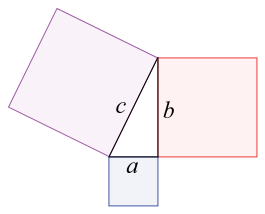
\includegraphics[scale=0.5]{pythagoras-1}
\end{floatingfigure}
Der \emph{Satz des Pythagoras} besagt: Errichtet man auf den drei Kanten eines
rechtwinkligen Dreiecks jeweils ein Quadrat, so sind die beiden kleineren
Quadrate zusammengenommen genauso groß wie das größte Quadrat (siehe Skizze
rechts). Als Formel:
\[ a \cdot a + b \cdot b = c \cdot c. \]
\emph{Wieso ist das so?} Das sollen die beiden anderen Skizzen beantworten.
Kannst du diesen Beweis erklären?
\begin{center}
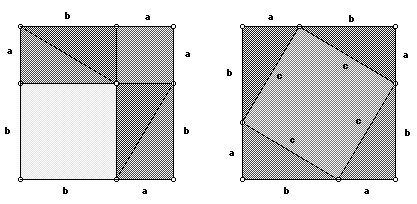
\includegraphics{pythagoras-2}
\end{center}

\vfill

\section*{Summe der natürlichen Zahlen I}
Was ist $1 + 2 + 3 + 4$? Was ist $1 + 2 + 3 + 4 + 5 + 6 + 7 + 8$? Das zu
berechnen, wird immer mühsamer. Zum Glück gibt es eine einfache Formel, die das
Ergebnis sofort liefert:
\begin{align*}
  1 + 2 + 3 + 4 + 5 + 6 + 7 + 8 &= 8 \cdot 9 : 2 \\
  1 + 2 + 3 + 4 + \cdots + 97 + 98 + 99 + 100 &= 100 \cdot 101 : 2
\end{align*}
Die Formel funktioniert auch mit jeder anderen Obergrenze als $100$. \emph{Wieso
stimmt die Formel?} Das soll die Skizze beantworten. Bei ihr ist die
Obergrenze~$6$. Kannst du den Beweis erklären?
\begin{center}
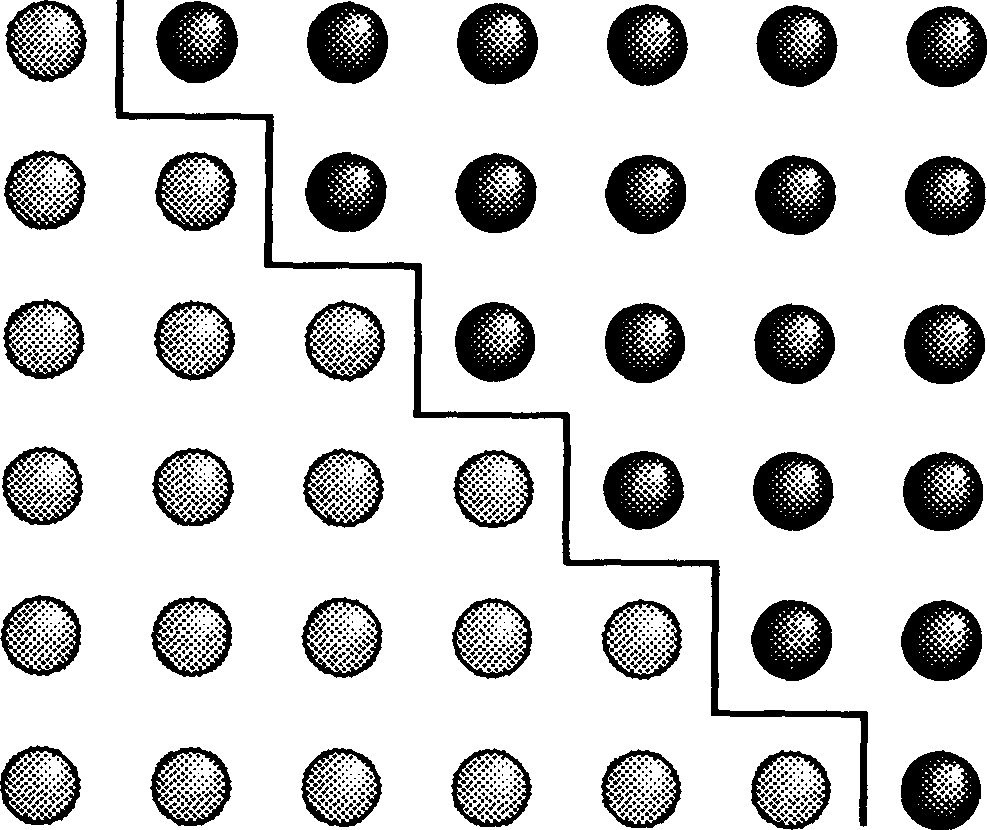
\includegraphics[scale=0.3]{kleiner-gauss-1}
\end{center}


\section*{Summe der natürlichen Zahlen II}
Was ist $1 + 2 + 3 + 4$? Was ist $1 + 2 + 3 + 4 + 5 + 6 + 7 + 8$? Das zu
berechnen, wird immer mühsamer. Zum Glück gibt es eine einfache Formel, die das
Ergebnis sofort liefert:
\begin{align*}
  1 + 2 + 3 + 4 + 5 + 6 + 7 + 8 &= 8 \cdot 9 : 2 \\
  1 + 2 + 3 + 4 + \cdots + 97 + 98 + 99 + 100 &= 100 \cdot 101 : 2
\end{align*}
Die Formel funktioniert auch mit jeder anderen Obergrenze als $100$. \emph{Wieso
stimmt die Formel?} Das soll die Skizze beantworten. Bei ihr ist die
Obergrenze~$100$. Kannst du den Beweis erklären?
\begin{center}
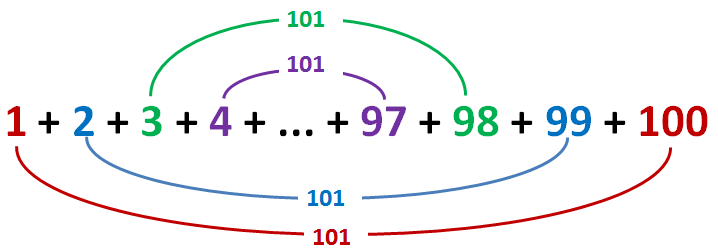
\includegraphics[scale=0.7]{kleiner-gauss-2}
\end{center}


\vfill
\section*{Summe der ungeraden Zahlen}
Was ist $1 + 3 + 5 + 7 + 9$? Was ist $1 + 3 + 5 + 7 + 9 + 11 + 13 + 15$? Das zu
berechnen, wird immer mühsamer. Zum Glück gibt es eine einfache Formel, die das
Ergebnis sofort liefert:
\begin{align*}
  1 + 3 + 5 + 7 + 9 + 11 \phantom{{} + 13 + 15} &= 6 \cdot 6 = 36 \\
  1 + 3 + 5 + 7 + 9 + 11 + 13 \phantom{{} + 15} &= 7 \cdot 7 = 49 \\
  1 + 3 + 5 + 7 + 9 + 11 + 13 + 15 &= 8 \cdot 8 = 64
\end{align*}
\emph{Wieso stimmt die Formel?} Das soll die Skizze beantworten. Kannst du
diesen Beweis erklären?
\begin{center}
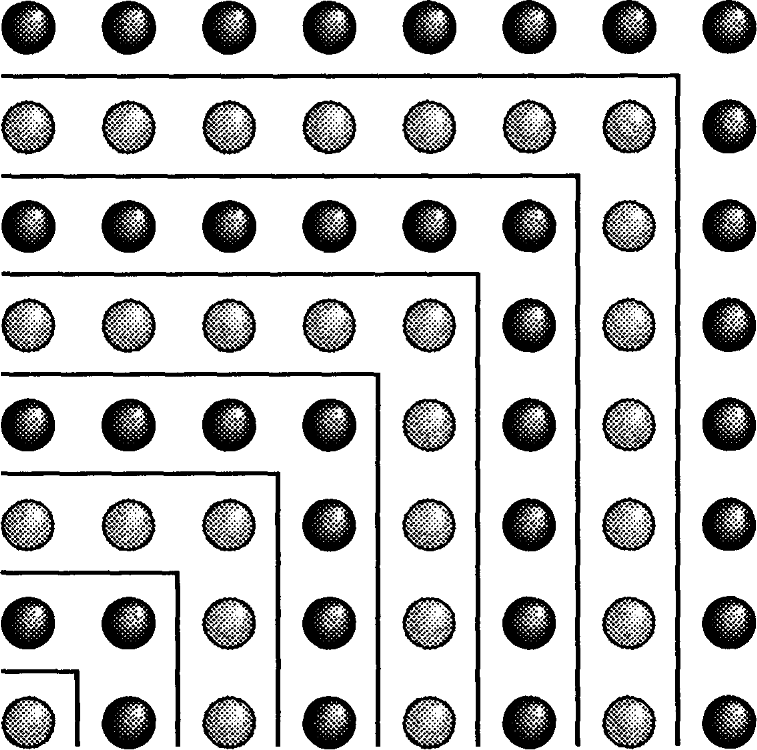
\includegraphics[scale=0.4]{summe-ungerade-zahlen}
\end{center}


\vfill
\section*{Summe der Fibonacci-Zahlen}

\end{document}

http://upload.wikimedia.org/wikipedia/commons/d/d2/Pythagorean.svg
http://jwilson.coe.uga.edu/EMT668/emt668.student.folders/HeadAngela/essay1/image1.gif
Proofs without Words, Seite 69
http://proofsfromthebook.com/wp-content/uploads/2013/01/sum-of-first-n-positive-integers.png
